\documentclass{article}
% Hebrew symbols
\usepackage[utf8]{inputenc}     % Allows UTF-8 characters
\usepackage[T1]{fontenc}        % Use T1 font encoding

%Algorithmics
\usepackage{algorithm}
\usepackage{float}
\usepackage{algpseudocode}
\usepackage{amsmath}

% Math, fonts, and symbols
\usepackage{amsmath, amssymb, amsfonts, mathtools, mathrsfs,  wasysym, {upgreek}, breqn}
\usepackage{physics}         % For derivatives, bras/kets, etc.
\usepackage{bm}              % Bold math symbols
\usepackage{cancel}          % Cancel terms with a line
\usepackage{siunitx}         % For scientific units like \SI{5}{\meter\per\second}
\usepackage{mathrsfs}        % Fancy math script font
\usepackage{dsfont}          % For double stroke 1 (like \mathds{1})

% Theorem environments
\usepackage{amsthm}
\newtheorem{theorem}{Theorem}
\newtheorem{definition}{Definition}
\newtheorem{lemma}{Lemma}

% Colors
\usepackage{xcolor}

% Others
\usepackage[spanish]{babel}
\usepackage{geometry}
\geometry{margin=1in}

% TikZ for diagrams
\usepackage{tikz}
\usetikzlibrary{3d}
\usepackage{tikz-3dplot}
\usetikzlibrary{arrows.meta, decorations.pathmorphing, positioning, shapes.geometric, calc, backgrounds, matrix}
\usepackage{pgfplots}
\pgfplotsset{compat=1.18}

% Optional:
\usepackage{graphicx}    % For including images
\usepackage{hyperref}    % For clickable links
\hypersetup{
    colorlinks=true,
    linkcolor=blue,
    urlcolor=cyan,
    citecolor=blue
}

\title{Tareas Matematicas para el Aprendizaje de Maquina}
\author{Santiago Forero Rosales}

\begin{document}
\maketitle
\tableofcontents
\newpage
\section{Tarea 1: Formula de la Entropia}
Por que $H(\mathcal X) = - \Sigma_{x \in \mathcal X} p(x) log \ p(x)$? \\ \\
\textbf{Solucion:} \\ \\
Consideremos $N$ como el numero de simbolos que tiene un mensaje considerablemente largo (un \textit{outcome} de la vida real). Sean $S = \{x_1,...,x_n\}$ el alfabeto sobre el cual esta cimentada la fuente que genera el mensaje, con distribucion de probabilidad (\textit{d.p.}) $\{p_1,...,p_n\}$ y $N_i$ el numero de veces que aparece el simbolo $x_i$. \\ \\
Por la \textbf{Ley del Producto}, cuando $N\gg1$, la frecuencia de ejemplares se aproxima a su valor esperado teorico \[
\lim_{N \to \infty} \frac{N_i}{N} = p_i,
\] por lo cual $N \sim N_i \cdot p_i$. Como tenemos una \textit{d.p}, $\Sigma_{i=1}^n \  p_i = 1$. De este modo, \[ \Sigma_{i=1}^n \ N_i = N \Sigma_{i=1}^n \ p_i = N.\]
Por otro lado, el coeficiente multinomial $W$ asociado a $S$ cuenta el numero de maneras de ordenar $N$ simbolos, donde cada $x_i$ aparece $N_i$ veces; su valor para nuestro caso es
\begin{align*}
    W &= \binom{N}{N_1} \binom{N-N_1}{N_2} \binom{N-N_1-N_2}{N_3} \cdots \binom{N- \Sigma_{i=1}^n N_i}{N_n} &\\ \\
    & = \frac{N!}{N_1! \ (N-N_1)!} \cdots \frac{(N-\Sigma_{i=1}^n N_i)}{N_n! \ (N-\Sigma_{i=1}^n N_i))!} &\\ \\
    &= \frac{N!}{N_1! \ N_2! \cdots N_n!} &\\ \\
    &= \frac{N!}{\Pi_{i=1}^n \ N_i!}.
\end{align*}
Ahora, necesitamos el siguiente lema: \\ \\
\textbf{\underline{Lema}:} Sea $a >1$. Entonces, existe una \textbf{unica} funcion creciente $f:(0, \infty) \longrightarrow \mathbb{R}$ tal que \\ \\
\hspace*{1cm} $(i) \ \ \ f(a) = 1,$ \\ 
\hspace*{1cm} $(ii) \ \ f(xy) = f(x) + f(y), \quad \forall x,y >0.$ \\ \\
\textbf{Demostracion:} \\ \\
Fijemos $x \in (0,1)$ arbitrario. Definimos $S_x = \left\{ \frac{k}{n} \in \mathbb{Q} \ | \ a^{\frac{k}{n}} \leq x \right\} \subseteq \mathbb{R}$.Este conjunto es no vacio, pues, por la \textbf{Desigualdad de Bernoulli}, para cualesquiera $h>0$ y $n \in \mathbb{N}$, se cumple \[(1+h)^n \geq 1 + nh.\] Sea $a=1+h$ para algun $h>0$ (este existe, una de las razones es que $a>1$), entonces  \[a^n \geq 1+nh > x\] (pues $x \in (0,1)$. De este modo, \[a^{-n} < x.\]
Asi, $-n \in S_x$ para todo $n \in \mathbb{N}$. Ademas, esta acotado superiormente (con el orden usual), pues, si $k\geq n$, entonces $\frac{k}{n} \geq 1$ de donde $\frac{k}{n} \not\in S_x$.  \\ \\
Definamos $f:(0,1) \longrightarrow \mathbb{R}$ dada por $f(x) = \sup S_x$. Nos damos cuenta que: \\ \\
\hspace{2cm} $(i)$ Cuando $x=a$, se cumple que $a^1 = a$, por lo cual $1 \in S_a$ y si $0<k<1$, entonces $k \in S_a$; ademas, si $k>1$, entonces $k \not\in S_a$. De este modo, $f(a) = \sup S_a 1$. \\ \\
\hspace{2cm} $(ii)$ $f(xy) = \sup S_{xy} = \sup \left\{ \frac{k}{n} \in \mathbb{Q} \ | \ a^{\frac{k}{n}} \leq xy \right\}$. Ahora bien, si $q \in S_x$ y $r \in S_y$, entonces $a^{q+r} = a^q a^r \leq xy$, lo que implica $q+r \in S_{xy}$, por lo tanto $S_x + S_y \subseteq S_{xy}$ y $\sup S_x + \sup S_y \leq \sup S_{xy}$. \\ \\ Inversamente, $\forall \epsilon > 0$, existen $q \in \mathbb{Q} \cap (f(x)-\epsilon, f(x)]$ y $r \in \mathbb{Q} \cap (f(y)-\epsilon, f(y)]$ tales que $a^{q+r} \leq xy$ es arbitrariamente cercano a $xy$. \\ \\
Ademas, $f$ es creciente. En efecto, \\ \\
Por la densidad de $\mathbb{Q}$ y la continuidad de $a^z$, resultando en $\sup S_{xy} \leq \sup S_x + \sup S_y$. 
Así, $f(xy) = \sup S_{xy} = \sup(S_x + S_y) = \sup S_x + \sup S_y = f(x) + f(y)$. \\ \\
Veamos ahora que, en efecto, esta funcion es unica. Razonando por reduccion al absurdo, supongamos que existe $x \in (0,1)$ tal que $f(x) \neq \sup S_x$. Necesitaremos mostrar por induccion que $f(x^n) = n f(x)$: \\ \\
\textbf{\underline{n=2}:} $f(x^2) = f(x \cdot x) = f(x) + f(x)$. \\ \\
\textbf{\underline{H.I}:} Supongamos que $f(x^{n-1}) = (n-1)f(x)$, para ciertos $n \in \mathbb{N}$. \\ \\
\textbf{\underline{P.I}:} Al realizar los calculos, tenemos que \[ f(x^n) = f(x^{n-1} \cdot x) = f(x^{n-1}) + f(x) = (n-1)f(x) + f(x) = nf(x). \] Asi, por el principio de induccion matematica, concluimos que $f(x^n) = nf(x)$ para todo $n \in \mathbb{Z}$. \\ \\
Veamos con ello la unicidad de $f$. Supongamos que existe $g: (0,1) \longrightarrow \mathbb{R}$ que cumple las mismas condiciones hipotesis. Dado $x \in (0, 1)$ y $\frac{k}{n} \in \mathbb{Q}$ con $n \in \mathbb{Q}$. \\ \\
Por el resultado anterior, $g(x^n) = ng(x)$, de donde $g(x^{-n}) = -ng(x)$ (pues $g(x) = g(y^n) = n g(y) = n g(x^{1/n})$ y por tanto,  $ g(x^{1/n}) = \frac{1}{n} g(x)$) y 
$g(x^{k/n}) = g(x) = \frac{k}{n} g(x)$ (pues $g(x^{k/n}) = g((x^{1/n})^k) = k g(x^{1/n}) = \frac{k}{n} g(x)$). \\ \\
Si 
$q = \frac{k}{n} \in S_x$, entonces 
$a^q \leq x \text{ implica } g(a^q) \leq g(x) \text{ que a su vez implica } q \cdot g(a) \leq g(x), \text{ de modo que } q \leq g(x)$, por lo cual 
$\sup S_x \leq g(x)$. \\ \\
Recíprocamente, si 
$q' \in \mathbb{Q}$ tal que 
$q' > f(x)$, entonces 
$a^{q'} > x \text{ por lo cual } g(a^{q'}) \geq g(x) \text{ y con esto, } q' \geq g(x)$, de donde 
$g(x) = \sup \{ q \in \mathbb{Q} \mid q \leq g(x) \} = f(x)$. \\ \\
Por lo tanto, 
$f = g$ es la única función que satisface las hipotesis. De este modo, $f(x) = \sup S_x = \log_a(x)$. De ahora en adelante, trabajaremos con $a=2$. \\ \\
Para representar la informacion, buscamos una funcion $I: S \longrightarrow C $ entre los dos conjuntos independientes de interes ($S$ fuente y $C$ destino), tales que $|S| = W_1$ y $|C| = W_2$. \\ \\ Por el \textbf{Axioma de Aditividad de Shannon-Khinchin}, sabemos que la informacion conjunta obtenida de dos sistemas independientes, es la suma de la informacion de cada una. Asi, $I(w_1 w_2) = I(w_1) + I(w_2)$. Esto nos dice que la funcion de informacion que buscamos es monotona creciente; en particular, como la concatenacion y la adicion son operaciones binarias, tenemos que  \[ I(w^k) = kI(w), \quad \forall k \in \mathbb{Z}^+.\]
Ahora, tomemos dos bases distintas $a,b \in \mathbb{R}$. Por la propiedad Arquimediana, para $m \gg 1$, podemos encontrar $n \in \mathbb{Z}^+$ tal que \[a^n \leq b^m < a^{n+1}.\]
Como $I$ es monotona creciente, tenemos que \[I(a^n) \leq I(b^m) < I(a^{n+1}),\] por lo cual \[nI(a) \leq mI(b) < (n+1) I(a),\] y con ello, \[\frac{n}{m} \leq \frac{I(b)}{I(a)} < \frac{n+1}{m}.\]
Por otro lado, de la desigualdad inicial, tenemos que \[\log (a^n) \leq  \log (b^m)< \log (a^{n+1}),\] lo cual implica que \[n \log (a) \leq m \log(b) < (n+1) \log(a),\] y asi, \[\frac{n}{m} \leq \frac{\log b}{\log a} < \frac{n+1}{m}.\]
De este modo, para $m \gg 1, \ \frac{1}{m} \ll 1$, de donde concluimos que $\frac{I(b)}{I(a)} \sim \frac{\log b}{\log a} \sim k \in \mathbb{R}$. Luego, $I(W) \sim \log(W)$ y, como vimos previamente, esto fuerza que $I$ se comporte como un logaritmo. \\ \\
Por otro lado, si la informacion total contenida en un mensaje de $N$ simbolos es $I$, la \textit{densidad de informacion} o \textit{informacion media} por simbolo es \[ \text{Inf.Prom.} = \frac{I}{N} = \frac{\log W}{N} \] y como previamente vimos que el numero de maneras de ordenar tales simbolos es \[W = \frac{N!}{\Pi_{i=1}^n \ N_i!} = \frac{N!}{\Pi_{i=1}^n \ (N \cdot p_i)},\] tenemos que \[\text{Inf.Prom.} = \frac{1}{N} \log \left( \frac{N!}{\Pi_{i=1}^n \ N_i!} \right). \] 
Ahora bien, si $A$ y $B$ son eventos independientes, tenemos que \[I[P(A \cap B)] = I[P(A) \cdot P(B)] = I[P(A)] + I[P(B)].\] Llamaremos, sin perdida de generalidad, $p_1:= p(A)$ y $p_2:= p(B)$; luego, \[I(p_1 \cdot p_2) = I(p_1) + I(p_2).\] Derivamos respecto a $p_2$, por lo cual \[\frac{d}{dp_2} [ I(p_1 \cdot p_2)] = \frac{d}{dp_2} [ I(p_1) + I(p_2)],\] de donde obtenemos \[p_1 I'(p_1\cdot p_2) = I'(p_2).\]
Sea $p_2 = 1$, entonces
\begin{align*}
    & \quad p_1  I'(p_1) = I'(1) &\\ \\
    & \implies I'(p_1) = \frac{I'(1)}{p_1} &\\ \\
    &  \implies \int I'(p_1) d p_1 = \int \frac{I'(1)}{p_1} dp_1 &\\ \\
    & \implies I(p_1) = I'(1) \log (p_1) + C.
\end{align*}
Ahora bien, si un evento es certero a ocurrir (p=1), este aporta cero informacion (pues ya sabemos lo que va a pasar). Luego,\[I(1) = I'(1) \ln(1) + C = 0+ C = 0,\] de lo cual tenemos que $C=0$. Ademas, la informacion debe incrementar a medida que la probabhilidad decrece (en virtud del Axioma de Maximalidad de Shannon-Khinchin Maximality) y como $\log p <0$ cuando $0 < p < 1$, tenemos que $I'(1)<0$ para que se cumpla $I(p)>0$. \\ \\
Sabemos, ademas, que $\log(x) < 0$ para cualquier $x \in (0,1)$, y ponderando con la distribucion de probabilidad, entonces $I'(1) = -1$. Asi, $I(p) = - \log (p)$. \\ \\
Recordando la \textbf{formula de Stirling} $\ln m! = m \ln m - m + O(\ln m)$, tenemos que
\begin{align*}
    \text{Inf.Prom.} &= \frac{1}{N} \log W &\\ \\
    &= \frac{1}{N} \left[ \log N! - \Sigma_{i=1}^n \log (N p_i)! \right] &\\ \\
    & = \frac{1}{N} \left[ N \log N - N - \Sigma_{i=1}^n (Np_i \log (Np_i) - Np_i) \right] &\\ \\
    & = \frac{1}{N} \left[  N \log N - N - \Sigma_{i=1}^n N p_i \log N - \Sigma_{i=1}^n N p_i \log p_i  -  \Sigma_{i=1}^n Np_i \right] &\\ \\
    & = \frac{1}{N} \left[ N \log N - N - \Sigma_{i=1}^n N p_i \log p_1 - N \log N + N \right] &\\ \\
    & = - \frac{1}{N} \Sigma_{i=1}^n N p_i \log p_i &\\ \\
    & = - \Sigma_{i=1}^n p_i \log p_i.
\end{align*}
Por el \textbf{Teorema de Khinchin}, sabemos que $H(X)$ es la \textit{unica} y \textit{necesaria} medida para la tasa de informacion promedio (es decir, la media de informacion). Ademas, pequenos cambios en $H(X)$ implican pequenos cambios en $p_i$, para $i = 1, ... , n$, por lo cual utilizaremos el siguiente resultado (que no mostraremos, pues sale del proposito del ejercicio): \\ \\
\textbf{\underline{Teorema} (Ley Debil de los Numeros Grandes):} \\
Dada una sucesion $\{X_n\}$ de muestras independientes e identicamente distribuidas ($i.i.d$) de una variable aleatoria $X$ tal que $E(X) = a \in \mathbb{R}$, existe $\varepsilon >0$ tal que \[ \lim_{n \longrightarrow \infty} P(|\overline{x_n}-a|< \varepsilon) = 1.\]
De este modo, si $Y$ modela la informacun de un evento $y_i = p_i \log p_i$, tenemos que $P(x_1,...,x_N) = \Pi_{i=1}^N \ p_i$ (pues son eventos independientes). Asi, \[ \frac{1}{N} \log P(x_1,...,x_N) = \frac{1}{N} \ \Sigma_{i=1}^n \log p_i\]. \\ 
Por la Ley Debil de los Numeros Grandes, tenemos que \[ \lim_{N \rightarrow \infty} P \left( \left| \frac{1}{N} \Sigma_{i=1}^N y_i - E[y] \gg \varepsilon \right| \right) =0 \] y como $y_i = p_i \log p_i$, entonces 
\begin{align*}
    H(X) &= \text{Inf.Prom.} &\\ 
    &= E[\log P(x_1,...,x_N)] &\\
    &= \frac{1}{N} \log W
\end{align*}
por lo cual, cuando $N \to \infty$,
\begin{align*}
    H(X) &= \lim_{N \to \infty} \frac{1}{N} \log W &\\ \\
    &= \lim_{N \to \infty} \frac{1}{N} \log \left( \frac{N!}{\Pi_{i=1}^n  (Np_i)!} \right) &\\ \\
    &= - \Sigma_{i=1}^n p_i \log p_i.
\end{align*}
\section{Tarea 2}
\subsection{Demostrar la desigualdad de Markov}
\noindent Para $X>0$ una variable aleatoria tal que $E(X) = \mu$ y $a >0$, mostrar que \[P(X \geq a) \leq \frac{E(X)}{a}.\]
\textbf{Demostracion:} Por definicion, $E[X] = \int_0^\infty x f(x) dx $; luego,
\begin{align*}
    E[X] &= \int_0^\infty x f(x) dx &\\ \\
    &= \int_0^a x f(x) dx + \int_a^\infty x f(x) dx &\\ \\ 
    & \geq \int_a^\infty a f(x) dx &\\ \\
    &= a \int_a^\infty f(x) dx &\\ \\
    &= a P(X \geq a).
\end{align*}
Ahora, si $X$ es discreta, tenemos que 
\begin{align*}
    E[X] &= \Sigma_x \ x \ P(X = x) &\\ \\
    &= \Sigma_{x<a} \ x \ P(X = x) + \Sigma_{x \geq a} \ x \ P(X = x)  &\\ \\
    & \geq \Sigma_{x \geq a} \ x \ P(X=x) &\\ \\
    & \geq \Sigma_{x \geq a} \ a \ P(X=x) &\\ \\
    &= a \Sigma_{x \geq a} \ P(X=x) &\\ \\
    &= a \ P(X\geq a).
\end{align*}
\subsection{Demostrar la desigualdad de Chebyshev}
\noindent Sea $X$ una variable aleatoria con $E[X] = \mu \in \mathbb{R}$ y $\mathrm{Var}(X) \in \mathbb{R}$. Entonces, para cualquier $a>0$, \[P(|X - \mu | \geq a) \leq \frac{\mathrm{Var}(X)}{a^2}.\]
\textbf{Demostracion:} Sea $X$ una variable aleatoria, entonces $(X - E[X])^2 \geq 0$ tambien es variable aleatoria (pues desplazamientos y elevar al cuadrado preservan aleatoridad). Aplicando la desigualdad de Markov, tenemos que
\begin{align*}
    P(|X - E[X]| \geq a) 
    &= P\left[(X-E[X])^2 \geq a^2\right] &\\ \\
    & \leq \frac{E\left[(X-E[X])^2\right]}{a^2} &\\ \\
    & = \frac{\mathrm{Var}(X)}{a^2}.
\end{align*}
\subsection{Demostrar la desigualdad de Hoeffding}
\noindent Sea $X$ una variable aleatoria que se puede expresar como la suma de $N$ variables aleatorias independientes, cada una acotada en el intervalo $[l_i,u_i]$: \[X = \Sigma_{i=1}^n X_i.\] Entonces, para cualquier $a>0$, \[P(|X-E[X]|>a) \leq e^{-\frac{2a^2}{\Sigma_{i=1}^N \ (u_i - l_i)}}.\]
\textbf{Demostracion:} 
Sea $X$ una variable aleatoria tal que $X = \sum_{i=1}^N X_i$, donde las $X_i$ son variables aleatorias independientes y cada una está acotada en el intervalo $[l_i, u_i]$. Necesitaremos algunos lemas:
\begin{lemma}[Lema de Hoeffding para una variable]
Sea $Z$ una variable aleatoria tal que $Z \in [l, u]$. Entonces para cualquier $\lambda \in \mathbb{R}$:
\[ \mathbb{E}\left[ e^{\lambda(Z - \mathbb{E}[Z])} \right] \leq \exp\left( \frac{\lambda^2(u - l)^2}{8} \right) \]
\end{lemma}
\begin{lemma}[Cota de Chernoff]
Para cualquier variable aleatoria $Y$ y cualquier $\lambda > 0$:
\[ P(Y \geq a) \leq e^{-\lambda a} \mathbb{E}[e^{\lambda Y}] \]
\end{lemma}
\begin{proof}
Definamos la variable centrada $S = X - \mathbb{E}[X] = \sum_{i=1}^N (X_i - \mathbb{E}[X_i])$. \\ \\
\textbf{Paso 1:}
Debido a la independencia de las variables $X_i$, la MGF de la suma es el producto de las MGF individuales:
\[
\mathbb{E}[e^{\lambda S}] = \mathbb{E}\left[ e^{\lambda \sum_{i=1}^N (X_i - \mathbb{E}[X_i])} \right] = \prod_{i=1}^N \mathbb{E}\left[ e^{\lambda (X_i - \mathbb{E}[X_i])} \right]
\]
Aplicando el \textbf{Lema 1} a cada término del producto:
\[
\mathbb{E}[e^{\lambda S}] \leq \prod_{i=1}^N \exp\left( \frac{\lambda^2 (u_i - l_i)^2}{8} \right) = \exp\left( \frac{\lambda^2 \sum_{i=1}^N (u_i - l_i)^2}{8} \right)
\]
\textbf{Paso 2:}
Para la cola superior, por el \textbf{Lema 2}:
\[
P(S \geq a) \leq e^{-\lambda a} \mathbb{E}[e^{\lambda S}] \leq \exp\left( \frac{\lambda^2 \sum_{i=1}^N (u_i - l_i)^2}{8} - \lambda a \right)
\]
\textbf{Paso 3:}
Para obtener la cota más ajustada, minimizamos el exponente respecto a $\lambda$. Sea $g(\lambda) = \frac{\lambda^2 \sum (u_i - l_i)^2}{8} - \lambda a$. Derivando e igualando a cero:
\[
g'(\lambda) = \frac{2\lambda \sum (u_i - l_i)^2}{8} - a = 0 \implies \lambda^* = \frac{4a}{\sum_{i=1}^N (u_i - l_i)^2}
\]
Sustituyendo $\lambda^*$ en la desigualdad:
\[
P(X - \mathbb{E}[X] \geq a) \leq \exp\left( -\frac{2a^2}{\sum_{i=1}^N (u_i - l_i)^2} \right)
\]
\textbf{Paso 4:}
Por simetría, la cola inferior $P(X - \mathbb{E}[X] \leq -a)$ tiene la misma cota. Usando el límite de la unión, concluimos que
\[
P(|X - \mathbb{E}[X]| \geq a) \leq 2\exp\left( -\frac{2a^2}{\sum_{i=1}^N (u_i - l_i)^2} \right)
\]
\end{proof}
\section{Tarea 3: Support Vector Machine}
Consultar en \hyperlink{https://colab.research.google.com/drive/1PkO9KV9lTNLd1QfVFIFTe7x3J4I-Q_pE?usp=sharing}{Cuaderno con SVM}.
\section{Tarea 4: Articulo}
\noindent Responder detalladame como se logro resolver el reto netflix a partir de la solucion del problema de factorizacion de matrices NO negativas (Sugerencia: Hacer un paralelo de Temas vs Tematicas  y de Tematicas vs Peliculas; deducir como es el comportamiento de la factorizacion a partir de este paralelo). \\ \\
\textbf{Analisis:} 
El problema se aborda mediante la reducción de una matriz de calificaciones dispersa $W \in \mathbb{R}^{m \times n}$, donde $m$ es el número de usuarios y $n$ el de películas. El objetivo es proyectar tanto a usuarios como a ítems en un espacio latente común de dimensión $k \ll \min(m, n)$. Matemáticamente, esto se traduce en encontrar una aproximación de rango bajo que capture las estructuras semánticas (temáticas) subyacentes. \\ \\
La aproximación se fundamenta en el teorema de SVD, que descompone la matriz original como $W \approx U \Sigma V^{T}$. En este contexto, $U \in \mathbb{R}^{m \times k}$ es una matriz ortogonal cuyas filas representan vectores de afinidad de los usuarios, $V \in \mathbb{R}^{n \times k}$ representa la pertenencia de las películas a los factores latentes, y $\Sigma \in \mathbb{R}^{k \times k}$ es una matriz diagonal que contiene los valores singulares que ponderan la importancia de cada dimensión latente. \\ \\
Cada entrada $w_{ij}$ de la matriz reconstruida se calcula mediante el producto escalar de los vectores latentes: $\hat{w}_{ij} = \sum_{r=1}^{k} \sigma_r u_{ir} v_{jr}$. Esta estructura permite modelar la interacción usuario-película a través de un "puente" de $k$ variables ocultas, similar a la lógica de la Factorización de Matrices No Negativas (NMF), donde los componentes son interpretables como características temáticas. \\ \\
A diferencia de un SVD estándar, el reto presentaba un sesgo en el muestreo. Si $p_{ij}$ es la probabilidad de que el par $(i, j)$ sea observado, la matriz de observaciones no es un reflejo directo de la población total. Ignorar esto conduciría a estimadores sesgados. Por ello, se introduce una corrección basada en la estructura marginal de las calificaciones. \\ \\
El ajuste del modelo no minimiza la norma de Frobenius convencional $\|W - \hat{W}\|_F^2$, sino una variante ponderada por la raíz cuadrada de las probabilidades de muestreo. El objetivo es minimizar la función de costo:
\[ J = \sum_{i,j} p_{ij} (w_{ij} - \hat{w}_{ij})^2 \]
Esto equivale a aplicar SVD sobre una matriz transformada donde cada entrada se escala por $\sqrt{p_{ij}}$, enfocando el error en las celdas con mayor relevancia estadística. \\ \\
Dada la alta dimensionalidad de $W$, el cálculo de los autovalores y autovectores se realiza mediante el algoritmo de Lanczos. Este es un método iterativo para encontrar valores propios de matrices grandes y dispersas, optimizando el tiempo de cómputo al trabajar en subespacios de Krylov, lo cual es esencial para manejar la escala del KDD Cup. \\ \\
La selección del rango $k=10$ actúa como una técnica de regularización. Un valor de $k$ demasiado alto permitiría al modelo memorizar el ruido de la matriz de entrenamiento (varianza alta), mientras que un $k$ bajo podría no capturar patrones complejos (sesgo alto). La observación de los autores sobre el sobreajuste justifica la restricción de la complejidad del modelo. \\ \\
Además del SVD, se incorporan métodos basados en vecindad, como la similitud ítem-ítem. Esto se formaliza mediante el coseno ajustado, donde la similitud entre dos películas $j$ y $l$ se define como:
\[ \text{sim}(j, l) = \frac{\sum_{i \in U_{jl}} (w_{ij} - \bar{w}_i)(w_{il} - \bar{w}_i)}{\sqrt{\sum (w_{ij} - \bar{w}_i)^2} \sqrt{\sum (w_{il} - \bar{w}_i)^2}} \]
corregido estadísticamente para evitar sesgos por pocas observaciones comunes. \\ \\
La predicción final $\hat{Y}$ no depende de un único modelo, sino de una combinación lineal de cuatro estimadores:
\[ \hat{Y} = \beta_0 + \beta_1 X_{base} + \beta_2 X_{SVD} + \beta_3 X_{similitud} + \beta_4 X_{reglas} \]
Donde $\beta_2 = 0.1987$ representa el peso otorgado al factor latente. Esta técnica de ensamble (o \textit{blending}) reduce el error de generalización al promediar las debilidades de cada aproximación individual. \\ \\
La métrica de éxito es el Error Cuadrático Medio Raíz (RMSE):
\[ \text{RMSE} = \sqrt{\frac{1}{N} \sum_{t=1}^{N} (y_t - \hat{y}_t)^2} \]
El logro de un RMSE de $0.256$ frente a modelos triviales ($0.279$) valida matemáticamente que la descomposición en factores latentes es capaz de extraer señales significativas de datos altamente ruidosos y dispersos.
\section{Tarea 5: K-Nearest-Neighbours}
\noindent Cual es el conjunto de hipotesis del modelo de aprendizaje \textit{K-Nearest Neighbours}? Cual es su modelo de aprendizaje? \\ \\
\textbf{Analisis:} \\ \\
El conjunto de hipótesis $\mathcal{H}$ en un modelo $K$-NN está intrínsecamente ligado a la geometría del espacio métrico $(\mathbb{R}^d, d)$. Para $K=1$, la hipótesis induce una teselación de Voronoi donde el espacio se particiona en regiones $\mathcal{R}_i = \{x \in \mathbb{R}^d : d(x, x_i) \leq d(x, x_j) \forall j \neq i\}$, siendo $x_i$ un vector del conjunto de entrenamiento $\mathcal{D}$. Para un $K$ arbitrario, la función de decisión $\hat{f}(x)$ se define como la agregación local $\text{mode}\{y_i\}_{i \in N_K(x)}$ para clasificación o $\frac{1}{K} \sum_{i \in N_K(x)} y_i$ para regresión, donde $N_K(x)$ es el conjunto de los $K$ índices de los vectores más cercanos a $x$. Esta aproximación representa una función constante por pedazos cuya complejidad, medida a través de la dimensión VC, es inversamente proporcional a $K$, permitiendo una adaptación no paramétrica a la topología de la distribución subyacente de los datos. \\ \\ 
Desde la perspectiva de la teoría de la computación, el algoritmo KNN opera bajo un paradigma de \textit{lazy learning}, donde la fase de entrenamiento se reduce a una operación de complejidad temporal $\mathcal{O}(1)$ (almacenamiento en memoria de $\mathcal{D}$). La inducción no produce un modelo paramétrico explícito $\theta$, sino que delega el costo computacional a la fase de consulta (inferencia). Matemáticamente, la estimación de la función objetivo en un punto de consulta $x_q$ requiere evaluar un funcional de distancia $d(x_q, x_i)$ sobre la totalidad del conjunto de soporte, resultando en una complejidad de búsqueda de $\mathcal{O}(nd)$ en su forma ingenua. Al no existir una minimización de una función de pérdida global durante el entrenamiento, el modelo realiza una aproximación local de la esperanza condicional $E[Y|X=x]$, fundamentando su convergencia en el hecho de que, conforme $n \to \infty$ y $K/n \to 0$, el error del vecino más cercano se aproxima asintóticamente a no más del doble del error de Bayes.
\section{Tarea 6: Aprendizaje Supervisado}
\noindent En aprendizaje supervisado, por que partimos de la suposicion de trabajar con un conjunto de entrenamiento de ejemplares independientes e identicamente distribuidos (IID)?\\ \\
\textbf{Analisis:} La suposición de que los datos \[\mathcal{D} = \{(x_i, y_i)\}_{i=1}^n\] son Independientes e Idénticamente Distribuidos (IID) permite la factorización de la densidad conjunta del conjunto de datos en el producto de sus densidades marginales: \[P(\mathcal{D}) = \prod_{i=1}^n P(x_i, y_i).\] En el marco de la Estimación de Máxima Verosimilitud (MLE), esta propiedad transforma el problema de optimización de una densidad conjunta de $n$ dimensiones en la maximización de la suma de log-verosimilitudes individuales: \[\hat{\theta} = \arg\max_{\theta} \sum_{i=1}^n \log P(x_i, y_i | \theta).\] A nivel tecnico, la independencia elimina los términos de covarianza y dependencia condicional cruzada entre observaciones, reduciendo la complejidad computacional de un crecimiento exponencial a una relación lineal $\mathcal{O}(n)$ respecto al tamaño de la muestra, garantizando la viabilidad del entrenamiento en espacios de parámetros de alta dimensionalidad. \\ \\
La asunción IID es el fundamento de la Minimización del Riesgo Empírico (ERM), ya que asegura que la muestra de entrenamiento es representativa de la población total $P(X,Y)$. Bajo esta premisa, el riesgo empírico \[R_{emp}(f) = \frac{1}{n} \sum_{i=1}^n \mathcal{L}(f(x_i), y_i)\] se comporta como un estimador insesgado del riesgo teórico \[R(f) = \mathbb{E}_{(X,Y)\sim P}[\mathcal{L}(f(X), Y)].\] De acuerdo con la Ley Fuerte de los Grandes Números y los resultados de Vapnik-Chervonenkis, se garantiza la convergencia uniforme: \[P(\sup_{f \in \mathcal{H}} |R_{emp}(f) - R(f)| > \epsilon) \to 0\] cuando $n \to \infty$. Esta cota asegura que un modelo que minimiza eficazmente la pérdida sobre los datos observados tendrá, con alta probabilidad, un error de generalización acotado sobre datos no vistos, siempre que estos provengan de la misma distribución subyacente.
\section{Tarea 7: Perceptrones}
\noindent Exponer a detalle cual es el algoritmo de aprendizaje del modelo de aprendizaje basado en perceptrones. \\ \\
\textbf{Analisis:} El Perceptrón establece un modelo de clasificación binaria mediante un hiperplano separador en $\mathbb{R}^d$ definido por la ecuación afín \[f(x) = w^T x + b.\] La hipótesis de decisión se formaliza mediante la función de activación signo, \[\hat{y} = \text{sgn}(w^T x + b),\] la cual mapea el espacio de entrada a etiquetas discretas $y \in \{-1, +1\}$. Matemáticamente, el objetivo es minimizar el cardinal del conjunto de muestras mal clasificadas $\mathcal{M}$, pero dado que dicha función es discontinua, el algoritmo utiliza el criterio de error del Perceptrón: \[L(w, b) = -\sum_{i \in \mathcal{M}} y_i (w^T x_i + b).\] Esta función de costo es continua y convexa por trozos, y representa la suma de las distancias funcionales de las observaciones erróneas al hiperplano de decisión. \\ \\
La minimización del riesgo empírico $L(w, b)$ no se realiza de forma analítica global, sino mediante Descenso de Gradiente Estocástico. Para cada instancia $(x_i, y_i)$ que satisface la condición de error \[y_i (w^T x_i + b) \leq 0\], el algoritmo calcula el gradiente local de la pérdida, resultando en \[\nabla_w L = -y_i x_i\] y \[\nabla_b L = -y_i.\] Aplicando una tasa de aprendizaje $\eta \in (0, 1]$, obtenemos las reglas de actualización vectorial: \[w^{(t+1)} = w^{(t)} + \eta y_i x_i\] y \[^{(t+1)} = b^{(t)} + \eta y_i.\] El álgebra lineal nos dice que cada actualización suma una fracción del vector de características al vector de pesos, rotando el hiperplano hacia una orientación que incrementa el margen funcional de la muestra errónea hasta corregir su clasificación. \\ \\
La estabilidad computacional del algoritmo está supeditada a la estructura de los datos. Según el Teorema  de Novikoff (o de Convergencia del Perceptrón), si el conjunto de datos es linealmente separable, existe un hiperplano óptimo con un margen geométrico $\gamma > 0$ tal que \[y_i (w^{*T} x_i) \geq \gamma.\] En este escenario, el número total de correcciones $k$ está acotado superiormente por $k \leq \frac{R^2}{\gamma^2}$, donde $R = \max \|x_i\|$ es el radio de la bola que contiene los datos. \\ \\Esta cota garantiza que el algoritmo alcanzará el error cero en tiempo constante. Por el contrario, en presencia de ruido o datos no separables ($\gamma \leq 0$), el algoritmo entra en un ciclo de oscilación infinita, lo que requiere la implementación de mecanismos de estabilidad como el algoritmo \textit{Pocket}. En este, Al fijar un límite de iteraciones $T_{max}$, se garantiza que el resultado final \[w_{final} = \hat{w}_{pocket}^{(T_{max})}\] sea, por construcción, el mejor candidato dentro del subespacio de parámetros explorado. Aunque no garantiza alcanzar el óptimo global absoluto en tiempo polinomial, asegura que el error de entrenamiento $\epsilon$ será menor o igual al error de cualquier otro estado visitado, proporcionando una solución robusta frente al ruido y al solapamiento de clases. Para finalizar esta tarea, quise poner el pseudocodigo del algoritmo que acabamos de discutir y del perceptron tambien, ayudandome de ChatGPT para su creacion en base a la discusion realizada.

\begin{algorithm}
\caption{Algoritmo Pocket (Variante Estable del Perceptrón)}
\begin{algorithmic}[1]

\State \textbf{Input:} Conjunto de datos
$\mathcal{D}=\{(x_i,y_i)\}_{i=1}^{n}$,
tasa de aprendizaje $\eta$,
máximo de iteraciones $T_{\max}$

\State \textbf{Iteration:}
$w^{(0)}\gets\mathbf{0}$; \ 
$\hat{w}_{\text{pocket}}\gets w^{(0)}$; \ 
$E_{\min}\gets \operatorname{contar\_errores}(w^{(0)},\mathcal{D})$

\For{$t=1$ \textbf{to} $T_{\max}$}

    \State Seleccionar $(x_i,y_i)$ mal clasificado tal que
    $\operatorname{sgn}\!\left((w^{(t-1)})^{T}x_i\right)\neq y_i$

    \State
    $w^{(t)}\gets
    w^{(t-1)}+\eta y_i x_i$

    \State
    $E_{\text{actual}}\gets
    \operatorname{contar\_errores}(w^{(t)},\mathcal{D})$

    \If{$E_{\text{actual}}<E_{\min}$}
        \State
        $\hat{w}_{\text{pocket}}\gets w^{(t)}$

        \State
        $E_{\min}\gets E_{\text{actual}}$

    \EndIf

\EndFor

\State \textbf{Retornar:} $\hat{w}_{\text{pocket}}$

\end{algorithmic}
\end{algorithm}

\begin{algorithm}[H]
\caption{Algoritmo de Aprendizaje del Perceptrón Estocástico}
\label{alg:perceptron}

\begin{algorithmic}[1]
\Statex Conjunto de entrenamiento:
$\mathcal{D}=\{(x_1,y_1),(x_2,y_2),\ldots,(x_n,y_n)\}$,
donde $x_i\in\mathbb{R}^{d}$ y
$y_i\in\{-1,+1\}$

\Statex Tasa de aprendizaje:
$\eta\in(0,1]$

\Statex Número máximo de épocas:
$T_{\max}$

\Ensure
\Statex Vector de pesos:
$w\in\mathbb{R}^{d}$

\Statex Sesgo:
$b\in\mathbb{R}$

\State $w \gets \mathbf{0}$

\State $b \gets 0$

\State $t \gets 0$

\State $\mathit{convergido} \gets \mathrm{false}$

\While{$t<T_{\max}$ \textbf{and} \textbf{not} $\mathit{convergido}$}

    \State $\mathit{convergido} \gets \mathrm{true}$

    \State Permutar aleatoriamente
    $\{1,2,\ldots,n\}$

    \For{cada muestra $i\in\{1,2,\ldots,n\}$}

        \State
        $a_i \gets w^{T}x_i+b$
        \Comment{Equivalente a $\sum_{j=1}^{d} w_jx_{ij}+b$}

        \If{$y_i a_i \le 0$}

            \State
            $w \gets w+\eta y_i x_i$
            \Comment{Actualizar pesos}

            \State
            $b \gets b+\eta y_i$
            \Comment{Actualizar sesgo}

            \State
            $\mathit{convergido} \gets \mathrm{false}$
        \EndIf
    \EndFor
    \State
    $t \gets t+1$

\EndWhile

\State \Return $(w,b)$

\end{algorithmic}
\end{algorithm}

\section{Tarea 8: Imposibilidad de algoritmo universal}
\noindent Explicar detalladamente por que \textbf{NO} existe un algoritmo de aprendizaje universal para conjuntos de hipotesis arbitrariamente distintos. \\ \\
\textbf{Analisis:} 
Sea $\mathcal{X}$ un dominio de entrada de cardinalidad finita y $\mathcal{Y} = \{0, 1\}$ el espacio de etiquetas. Consideramos el conjunto $\mathcal{F} = \mathcal{Y}^{\mathcal{X}}$ de todas las posibles funciones objetivo. Un algoritmo de aprendizaje $\mathcal{A}$ se define como una aplicación que mapea un conjunto de entrenamiento $\mathcal{S} = \{(x_i, y_i)\}_{i=1}^m$ a una hipótesis $h \in \mathcal{Y}^{\mathcal{X}}$. \\ \\
El \textbf{Teorema del No Free Lunch} de Wolpert establece que, si el rendimiento de un algoritmo se mide por su error de generalización fuera de la muestra, el promedio de dicho error sobre todas las funciones $f \in \mathcal{F}$ es constante para cualquier $\mathcal{A}$. Formalmente:
 
\begin{equation}
\mathbb{E}_{\mathcal{F}} [L(f, \mathcal{A}(\mathcal{S}))] = \frac{1}{|\mathcal{F}|} \sum_{f \in \mathcal{F}} \sum_{x \notin \mathcal{S}} \mathbb{P}(f(x) \neq \mathcal{A}(\mathcal{S})(x)) = \frac{1}{2}
\end{equation}
Este resultado implica algo trascendental: por cada función para la cual un algoritmo $\mathcal{A}$ generaliza con éxito, existe una función dual donde el mismo algoritmo falla. En consecuencia, la superioridad de un modelo no es una propiedad intrínseca de su arquitectura, sino una manifestación de su alineación con la distribución subyacente. \\ \\
Establecida la imposibilidad de un aprendiz universal, la teoría del aprendizaje estadístico busca caracterizar las condiciones bajo las cuales un espacio de hipótesis $\mathcal{H}$ es ``PAC-aprendible'' (Probably Approximately Correct). Invocamos la \textbf{Dimensión de Vapnik-Chervonenkis}, denotada como $\text{VC}(\mathcal{H})$, que define la capacidad combinatoria de $\mathcal{H}$ para fragmentar (shatter) subconjuntos de $\mathcal{X}$. De acuerdo con el \textbf{Teorema Fundamental del Aprendizaje Estadístico}, una condición necesaria y suficiente para la convergencia uniforme del error es que $\text{VC}(\mathcal{H}) < \infty$. Para una muestra de tamaño $m$, el riesgo real $R(h)$ se encuentra acotado superiormente por el riesgo empírico $\hat{R}_m(h)$ mediante la desigualdad:
\begin{equation}
R(h) \leq \hat{R}_m(h) + \sqrt{\frac{8 d \ln(2em/d) + 8 \ln(4/\delta)}{m}}
\end{equation}
\noindent donde $d = \text{VC}(\mathcal{H})$ y $1-\delta$ es el nivel de confianza. Si un algoritmo intentara operar sobre la totalidad de $\mathcal{F}$, se tendría $d \to \infty$, lo que anularía la convergencia de la cota de error. Por tanto, el aprendizaje es teoricamente factible, si y solo si, se restringe la complejidad del espacio de búsqueda. \\ \\
Desde la perspectiva de la computación algorítmica, la selección de la hipótesis óptima se formula como un problema de \textbf{Minimización del Riesgo Estructural} (SRM). Dado que la minimización del error empírico puro es un problema NP-duro para clases de hipótesis generales, el algoritmo implementa un sesgo inductivo a través de un funcional de regularización $\Omega(h)$. El proceso de optimización se define como:
 
\begin{equation}
h^* = \arg \min_{h \in \mathcal{H}} \left\{ \frac{1}{m} \sum_{i=1}^m \ell(h(x_i), y_i) + \lambda \|h\|_{\Omega} \right\}
\end{equation}
\noindent donde $\ell$ es la función de pérdida y $\lambda$ es el parámetro de penalización. Este esquema revela que el algoritmo no ``descubre'' conocimiento de forma pura, sino que proyecta las restricciones impuestas por $\Omega(h)$ —tales como la suavidad, la parsimonia (Norma $L_1$) o la invarianza topológica— sobre los datos. La eficiencia computacional se adquiere, por tanto, mediante la renuncia a la universalidad, transformando el aprendizaje en un ejercicio de optimización restringida. \\ \\
Concluimos que la generalización es una transferencia de información desde el sesgo inductivo hacia la interpretación de la muestra. Por el \textbf{Lema Fundamental del Aprendizaje}, para cualquier algoritmo de aprendizaje $A$ y cualquier tamaño de muestra $m \leq d/2$, existe una distribución de probabilidad sobre $\mathcal{X} \times \mathcal{Y}$ tal que el error esperado de $A$ es al menos $1/4$, a pesar de que existe una hipótesis en $\mathcal{H}$ con error cero. \\ \\
Esto demuestra que sin una estructura de regularidad estadística asumida a priori, la optimización deviene en una mera interpolación de ruido. La frontera epistemológica del aprendizaje reside en esta dualidad: no existe (por el momento) la piedra filosofal del aprendizaje, pues la capacidad de extraer leyes generales de la realidad física depende estrictamente del ingenio para acotar el espacio de posibilidades mediante hipótesis coherentes y estructuralmente finitas. En última instancia, el aprendizaje no es la ausencia de límites, sino la aplicación estratégica de los mismos, razon por la cual la existencia de un limite determinisitco de estas capacidades es sinceramente absurdo.
\section{Tarea 9: Perceptrones en distribuciones Gaussianas}
\noindent Construir un modelo de distribuciones Gaussianas en el plano e implementar en el modelo el algoritmo de perceptrones. \\ \\ 
\textbf{Solucion:} Redirigirse al siguiente \hyperlink{https://colab.research.google.com/drive/1VsHPskZ8GEHAOjnnoC54lV5ICCNrOiIC?usp=sharing}{cuaderno} para la solucion.
\section{Tarea 10: Perceptrones V.2}
\noindent Respecto al Algoritmo de Aprendizaje de Perceptrones (previamente introducido en la Tarea 7), el algoritmo encuentra los parametros correctos (bajo que precision)? El algoritmo para en un numero finito de pasos? Por que funciona este algoritmo? Verificar que converge. \\ \\
\textbf{Analisis:} El  Algoritmo de Aprendizaje de Perceptrones (PLA) funciona porqu, para cada actualizacion, el conjunto hipotesis acepta separabilidad lineal. Este Algoritmo garantiza un riesgo empírico nulo en datos linealmente separables:
$$R_{emp}(w) = 0 \iff \forall i \in \{1, \dots, n\}: y_i(w^{*T}x_i + b^*) > 0$$
\textbf{Nota:} La solución $w^*$ no es única y no maximiza el margen, lo que limita la precisión de generalización. \\ \\
Bajo separabilidad lineal (hipotesis fundamental), existe $w^*$ con $\|w^*\| = 1$ y margen $\gamma > 0$ tal que $y_i(w^{*T}x_i) \geq \gamma$. El número máximo de actualizaciones $t$ está acotado por:
$$t \leq \left\lfloor \left( \frac{R}{\gamma} \right)^2 \right\rfloor, \quad R = \max_i \|x_i\|$$ \\ \\
Si $y_i(w^{(t)T}x_i) \leq 0$, se aplica la regla $w^{(t+1)} = w^{(t)} + y_i x_i$. Esto garantiza un ajuste direccional correcto:
$$y_i(w^{(t+1)T}x_i) = y_i(w^{(t)T}x_i) + y_i^2\|x_i\|^2 > y_i(w^{(t)T}x_i)$$ \\ \\
Partiendo de $w^{(0)} = 0$, se establecen dos cotas tras $t$ pasos:
\begin{enumerate}
    \item $w^{*T}w^{(t)} \geq t\gamma$ (Crecimiento lineal del producto escalar).
    \item $\|w^{(t)}\|^2 \leq tR^2$ (Crecimiento sublineal de la norma).
\end{enumerate}
Por desigualdad de Cauchy-Schwarz:
$$t\gamma \leq w^{*T}w^{(t)} \leq \|w^*\| \|w^{(t)}\| \leq 1 \cdot \sqrt{t}R$$
$$t^2\gamma^2 \leq tR^2 \implies t \leq \left( \frac{R}{\gamma} \right)^2.$$ Esta resulta ser la precision (no deterministica) de convergencia del PLA. Ademas, verifica que termina en un numero finito de pasos. 
\section{Tarea 11: Puntos de Juntura}
\noindent Determine los putnos de juntura de la shallow network modelada por la aplicacion \[y = f(x, \phi) = \phi_0 + \phi_1 a[\theta_{10} + \theta_{11}x] + \phi_2 a[\theta_{20} + \theta_{21}x] + \phi_3 a[\theta_{30} + \theta_{31}x].\] \textit{Sugerencia}: Los pesos quedan representados en la juntura. Que pasa siigualamos a cero cada uno (o todos) de los factores lineales?\\ \\
\textbf{Solucion:} La red definida por $f(x, \phi) = \phi_0 + \sum_{i=1}^3 \phi_i a[\theta_{i0} + \theta_{i1}x]$ opera como una función lineal continua por trozos (lo que se conoce como \textit{Continuous Piecewise Linear}). El conjunto de puntos de juntura $\mathcal{K} = \{x_i \in \mathbb{R} : x_i = -\theta_{i0}/\theta_{i1}\}$ define las singularidades de la primera derivada (cosa que ya mostraremos). En términos computacionales, cada $x_i$ marca una transición en el estado de activación de la unidad $i$, subdividiendo el dominio en regiones convexas donde el gradiente local $\frac{\partial f}{\partial x}$ permanece invariante. \\ \\
La capacidad de aproximación está sujeta a la cardinalidad de $\mathcal{K}$. Si se impone la condición de colapso $x_1 = x_2 = x_3$, la red sufre una degeneración de rango en su espacio latente, reduciendo el número de segmentos lineales de $n+1$ a 2. A nivel teorico, este fenómeno implica que los vectores de parámetros $\theta_i$ son linealmente dependientes en el espacio de las fases de activación, lo que fuerza a la salida $f(x)$ a converger al sesgo global $\phi_0$ en el punto de coincidencia, eliminando la capacidad del modelo para representar funciones de alta varianza local. \\ \\
La razon de por que finalmente esos terminan siendo los puntos de juntura, se fundamenta en la matriz Jacobiana $\mathbf{J} = \nabla_{\mathbf{\Theta}} f(x)$. Utilizando la función indicadora $\mathbb{I}(\cdot)$, las derivadas parciales se expresan como:
$$\frac{\partial f}{\partial \phi_i} = a[\theta_{i0} + \theta_{i1}x], \quad \frac{\partial f}{\partial \theta_{i0}} = \phi_i \mathbb{I}(\theta_{i0} + \theta_{i1}x > 0), \quad \frac{\partial f}{\partial \theta_{i1}} = \phi_i x \mathbb{I}(\theta_{i0} + \theta_{i1}x > 0)$$
Esta estructura implica que $\mathbf{J}$ es una función constante por tramos con discontinuidades en $\mathcal{K}$. La evaluación de $f(x, \phi)$ en los vértices permite la identificación algebraica de los pesos, dado que la nulidad del término $a[0]$ desacopla las contribuciones marginales de las neuronas en sus respectivos umbrales. \\ \\
Debido a la naturaleza no suave de ReLU, el paisaje de pérdida presenta aristas donde el gradiente no está definido. Usamos el algoritmo de retropropagación en ese caso, que utiliza el subgradiente, enfrentando discontinuidades de salto en cada $x_i \in \mathcal{K}$. Computacionalmente, esto significa que el vector de actualización de pesos muta de forma abrupta al cruzar una juntura, una propiedad que permite a la red modelar cambios de régimen nítidos pero que requiere esquemas de regularización para evitar oscilaciones en el proceso de minimización del riesgo empírico. \\ \\
Al sustituir la activación por funciones suaves $\sigma \in C^\infty$ (por ejemplo, Sigmoide), la red se transforma en una variedad diferenciable. Los puntos $x_i$ dejan de ser quiebres geométricos y pasan a ser puntos de inflexión donde la curvatura $\kappa = \frac{|f''|}{(1+f'^2)^{3/2}}$ alcanza sus valores críticos. En este paradigma, el Jacobiano es continuo en todo el dominio, lo que permite el uso de métodos de Newton o cuasi-Newton, aunque se pierde la propiedad de soporte compacto de la activación, extendiendo la influencia de cada parámetro $\theta_{ij}$ a través de todo el espacio de entrada.
\section{Tarea 12: Ejercicios presentacion perceptrones}
\noindent Realizar los ejercicios de la presentacion de Modelos de Aprendizaje. \\ \\
\textbf{Solucion:} Hay dos ejercicios, \\ \\
\emph{1.2. Supongamos que podemos usar un perceptron para detectar mensages spam. Asumamos tambien que cada mensaje es representado pro la frecuencia de ocurrencia de las palabras claves comunes en un correo spam, donde el output es +1 si el mensaje es spam. \begin{enumerate}
    \item Que palabras clave crees podrian tener mas peso positivo en el perceptron?
    \item Que palabras clave crees podrian tener peso negativo?
    \item Que parametro en el perceptron afecta directamente cuantos mensajes en la frontera de clasificacion terminan siendo clasificados como spam?
\end{enumerate}}
\textbf{Solucion:} \\ \\
\textit{1)} Sea un clasificador basado en un perceptrón definido por la función de decisión:
\[
f(\mathbf{x}) = \text{sgn}(\mathbf{w}^\top \mathbf{x} + b)
\]
donde:
\begin{itemize}
    \item $\mathbf{x} \in \mathbb{R}^n$ es el vector de entrada donde cada componente $x_i$ denota la frecuencia de la palabra clave $i$.
    \item $\mathbf{w} \in \mathbb{R}^n$ es el vector de pesos sinápticos.
    \item $b \in \mathbb{R}$ es el término de sesgo (bias).
\end{itemize}
Las palabras con mayor relevancia para la detección de \textit{spam} son aquellas cuyos pesos asociados cumplen que $w_i > 0$. Formalmente, el algoritmo de aprendizaje ajusta $\mathbf{w}$ de tal manera que:
\[
w_i \gg 0 \iff P(x_i > 0 \mid \text{spam}) \gg P(x_i > 0 \mid \text{legítimo})
\]
Consecuentemente, términos con alta frecuencia en mensajes de \textit{spam} aumentan la combinación lineal $\mathbf{w} \cdot \mathbf{x}$, favoreciendo la activación de la salida positiva del perceptrón. Consideremos un mensaje de spam con el vector de características 
\[\mathbf{x} = [x_{\text{gratis}}, x_{\text{oferta}}, x_{\text{reembolso}}]^\top = [3, 2, 1]^\top,\] donde las altas frecuencias de estas palabras clave interactúan con un vector de pesos entrenado 
$\mathbf{w} = [1,5, 1,2, 0,8]^\top$ y un sesgo 
$b = -2,0$. Al calcular la suma ponderada 
\[\mathbf{w} \cdot \mathbf{x} + b = (1,5 \cdot 3) + (1,2 \cdot 2) + (0,8 \cdot 1) - 2,0 = 4,5 + 2,4 + 0,8 - 2,0 = 5,7 \quad ,\] el resultado positivo activa la función de decisión 
$f(\mathbf{x}) = \text{sgn}(5,7) = +1$, validando que la acumulación de pesos positivos 
$w_i$ ante la presencia de términos como “gratis” desplaza el vector de forma efectiva hacia la clasificación de spam. \\ \\
\textit{2)} Consideremos el mismo modelo de clasificación binaria previa, donde la etiqueta $y = -1$ representa un mensaje legítimo. En este contexto, el vector de pesos $\mathbf{w}$ asigna valores $w_i < 0$ a las componentes $x_i$ orrespondientes a términos cuya probabilidad condicional es mayor en la clase legítima, es decir, 
\[P(x_i > 0 \mid y = -1) > P(x_i > 0 \mid y = +1).\] Esto quiere decir que, dado un mensaje representado por el vector de frecuencias $\mathbf{x}$, la presencia de palabras con $w_i < 0$ (como “saludo” o “consulta”) reduce la magnitud de la combinación lineal \[z = \mathbf{w}^\top \mathbf{x} + b,\] desplazando el valor hacia el semi-espacio negativo definido por el hiperplano de decisión. Por lo tanto, si 
\[\sum_{i: w_i < 0} w_i x_i\] es suficientemente pequeña, se garantiza que 
$f(\mathbf{x}) = \text{sgn}(z) = -1$, logrando una correcta inhibición de la clase spam. \\ \\
Para simular este comportamiento, consideremos un mensaje legítimo representado por el vector de características \[\mathbf{x} = [x_{\text{reunión}}, x_{\text{amigo}}, x_{\text{información}}]^\top = [1, 2, 1]^\top,\] donde la presencia de estos términos interactúa con un vector de pesos negativos $\mathbf{w} = [-1,8, -1,2, -0,5]^\top$ y un sesgo $b = 2,5$; al realizar el producto escalar y sumar el sesgo obtenemos \[\mathbf{w} \cdot \mathbf{x} + b = (-1,8 \cdot 1) + (-1,2 \cdot 2) + (-0,5 \cdot 1) + 2,5 = -1,8 - 2,4 - 0,5 + 2,5 = -2,2,\] lo que resulta en una activación $f(\mathbf{x}) = \text{sgn}(-2,2) = -1$, validando que el peso negativo de palabras como ``reunión'' es capaz de neutralizar el sesgo y clasificar correctamente el mensaje como legítimo. \\ \\
\textit{3)} El parámetro de sesgo $b \in \mathbb{R}$ determina la traslación del hiperplano de decisión definido por la ecuación:
\[
H_b = \{ \mathbf{x} \in \mathbb{R}^n : \mathbf{w}^\top \mathbf{x} + b = 0 \}
\]
En el clasificador $f(\mathbf{x}) = \text{sgn}(\mathbf{w}^\top \mathbf{x} + b)$, un incremento en el valor de $b$ reduce el umbral de activación para la clase \textit{spam} ($y = +1$). Formalmente, si definimos la región de decisión positiva como $R_+ = \{ \mathbf{x} : \mathbf{w}^\top \mathbf{x} > -b \}$, podemos ver que:
\[
b' > b \implies R_+(b) \subset R_+(b')
\]
Este desplazamiento expande el volumen del espacio de características asignado a la clase positiva, provocando que los vectores $\mathbf{x}$ en la frontera de clasificación sean etiquetados como \textit{spam}. Por lo tanto, $b$ regula directamente el compromiso (\textit{trade-off}) entre la exhaustividad (recall) y la tasa de falsos positivos del sistema. \\ \\
\emph{1.3. La regla de actualización de pesos en el algoritmo del perceptrón se define como:
\[
\mathbf{w}(t+1) = \mathbf{w}(t) + \alpha y(t) \mathbf{x}(t)
\]
donde:
\begin{itemize}
    \item $\mathbf{w}(t)$ es el vector de pesos en el instante $t$.
    \item $\alpha > 0$ es la tasa de aprendizaje (\textit{learning rate}).
    \item $y(t) \in \{-1, +1\}$ es la etiqueta real de la muestra $\mathbf{x}(t)$.
\end{itemize}
Esta regla posee la propiedad de ajustar el vector de pesos en la dirección que minimiza el error de clasificación para $\mathbf{x}(t)$. Demuestre lo siguiente:
\begin{enumerate}
    \item Muestre que $y(t) \mathbf{w}^\top(t) \mathbf{x}(t) < 0. \quad$ (\textit{Sugerencia:} $\mathbf{x}(t)$ es clasificado erróneamente por $\mathbf{w}(t)$).
    \item Muestre que $y(t) \mathbf{w}^\top(t+1) \mathbf{x}(t) > y(t) \mathbf{w}^\top(t) \mathbf{x}(t). \quad$ (\textit{Sugerencia:} Sustituya la regla de actualización de pesos en el término de la izquierda).
    \item En lo que respecta a la clasificación de $\mathbf{x}(t)$, argumente de manera formal si el paso de $\mathbf{w}(t)$ a $\mathbf{w}(t+1)$ constituye un movimiento en la ``dirección correcta''.
\end{enumerate}}
\textbf{Solucion:} \\ \\
\textit{1)} Si el vector $\mathbf{x}(t)$ es clasificado erróneamente por $\mathbf{w}(t)$, entonces el signo de la predicción $\text{sgn}(\mathbf{w}^\top(t)\mathbf{x}(t))$ es opuesto al signo de la etiqueta real $y(t)$:
\begin{align*}
    \text{Si } y(t) = +1 &\implies \mathbf{w}^\top(t)\mathbf{x}(t) < 0 &\\ \\
    \text{Si } y(t) = -1 &\implies \mathbf{w}^\top(t)\mathbf{x}(t) > 0 
\end{align*}
En ambos casos, $y(t) \left( \mathbf{w}^\top(t)\mathbf{x}(t) \right) < 0$. \\ \\
\textit{2)} Utilizando la regla de actualización $\mathbf{w}(t+1) = \mathbf{w}(t) + \alpha y(t) \mathbf{x}(t)$:
\begin{align*}
    y(t) \mathbf{w}^\top(t+1) \mathbf{x}(t) &= y(t) \left( \mathbf{w}(t) + \alpha y(t) \mathbf{x}(t) \right)^\top \mathbf{x}(t) &\\ \\
    &= y(t) \left( \mathbf{w}^\top(t) + \alpha y(t) \mathbf{x}^\top(t) \right) \mathbf{x}(t) &\\ \\
    &= y(t) \mathbf{w}^\top(t) \mathbf{x}(t) + \alpha y(t)^2 \mathbf{x}^\top(t) \mathbf{x}(t) &\\ \\
    &= y(t) \mathbf{w}^\top(t) \mathbf{x}(t) + \alpha (1) \|\mathbf{x}(t)\|^2 &\\ \\
    &> y(t) \mathbf{w}^\top(t) \mathbf{x}(t).
\end{align*}
Esto, pues $\alpha > 0$ y $\|\mathbf{x}(t)\|^2 > 0$ (asumiendo un vector no nulo). \\ \\
\textit{3)} Para que la clasificación sea correcta, se requiere que $y(t) \mathbf{w}^\top \mathbf{x}(t) > 0$. El movimiento es en la dirección correcta porque:
\begin{align*}
    \Delta \text{score} &= y(t) \mathbf{w}^\top(t+1) \mathbf{x}(t) - y(t) \mathbf{w}^\top(t) \mathbf{x}(t) &\\ \\
    &= \alpha \|\mathbf{x}(t)\|^2 &\\ \\
    &> 0.
\end{align*}
Este resultado positivo implica que el valor de la función de decisión se desplaza algebraicamente hacia la región de clasificación correcta (hacia valores positivos si $y=1$, o hacia valores más negativos si $y=-1$, lo que en el producto por $y(t)$ siempre resulta en un incremento). Por lo tanto, $\mathbf{w}(t+1)$ reduce el error cometido por $\mathbf{w}(t)$.
\section{Tarea 13: XOR vs Algoritmos de Aprendizaje}
\noindent Modelar un XOR conectando varias neuronas básicas. Luego modelar un XOR con perceptrones (con pesos específicos para cada uno). \\ \\
\textbf{Solucion:} Sea $H(z)$ la función de activación de Heaviside. El sistema se define mediante las siguientes etapas: \\ \\
La neurona $h_1$ representa la unión de los conjuntos de entrada: $z_1 = \mathbf{w}_1^\top \mathbf{x} + b_1$.
\begin{center}
\begin{tabular}{cccc}
\toprule
$x_1$ & $x_2$ & $z_1 = x_1 + x_2 - 0,5$ & $h_1 = H(z_1)$ \\
\midrule
0 & 0 & $-0,5$ & 0 \\
1 & 0 & $0,5$  & 1 \\
0 & 1 & $0,5$  & 1 \\
1 & 1 & $1,5$  & 1 \\
\bottomrule
\end{tabular}
\end{center}
La neurona $h_2$ representa la intersección de los conjuntos de entrada: $z_2 = \mathbf{w}_2^\top \mathbf{x} + b_2$.
\begin{center}
\begin{tabular}{cccc}
\toprule
$x_1$ & $x_2$ & $z_2 = x_1 + x_2 - 1,5$ & $h_2 = H(z_2)$ \\
\midrule
0 & 0 & $-1,5$ & 0 \\
1 & 0 & $-0,5$ & 0 \\
0 & 1 & $-0,5$ & 0 \\
1 & 1 & $0,5$  & 1 \\
\bottomrule
\end{tabular}
\end{center}
La neurona $\hat{y}$ proyecta el espacio $\{h_1, h_2\}$ a la salida final: $z_o = \mathbf{w}_o^\top \mathbf{h} + b_o$.
\begin{center}
\begin{tabular}{cccc}
\toprule
$h_1$ & $h_2$ & $z_o = h_1 - 2h_2 - 0,5$ & $\hat{y} = H(z_o)$ \\
\midrule
0 & 0 & $-0,5$ & 0 \\
1 & 0 & $0,5$  & 1 \\
1 & 1 & $-1,5$ & 0 \\
\bottomrule
\end{tabular}
\end{center}
Asi, al componer las funciones $f: \mathbb{B}^2 \to \mathbb{B}$, concluimos la convergencia al operador XOR:
\begin{center}
\begin{tabular}{cccccc}
\toprule
$x_1$ & $x_2$ & $h_1$ & $h_2$ & $\hat{y}$ & \textbf{XOR} \\
\midrule
0 & 0 & 0 & 0 & 0 & 0 \\
1 & 0 & 1 & 0 & 1 & 1 \\
0 & 1 & 1 & 0 & 1 & 1 \\
1 & 1 & 1 & 1 & 0 & 0 \\
\bottomrule
\end{tabular}
\end{center}
El grafico del primer caso sin usar perceptrones seria \\ \\
\textbf{Grafico} \\ \\
y usando perceptrones con pesos especificos, quedaria \\ \\
\begin{center}
\begin{tikzpicture}
\begin{axis}[
    width=8cm, height=8cm,
    xlabel={$x$}, ylabel={$y$},
    xmin=-0.3, xmax=1.3, ymin=-0.3, ymax=1.3,
    xtick={0,1}, ytick={0,1},
    axis lines=middle,
    legend pos=outer north east,
    legend style={font=\footnotesize}
]
\addplot[fill=orange!20, draw=none] coordinates {
     (0.7,0.2) (0.2,0.7)
} \closedcycle;

\addplot[blue, thick, domain=-0.005:0.9, samples=2] {0.9 - x};
\addlegendentry{Frontera de $h_1$(OR)}

\addplot[red, thick, domain=0.2:1.3, samples=2] {1.5 - x};
\addlegendentry{Frontera de $h_2$ (AND)}

\addplot[only marks, mark=*, mark size=3pt, gray] coordinates {(0,0) (1,1)};
\addlegendentry{XOR = 0}
\addplot[only marks, mark=*, mark size=3pt, teal] coordinates {(1,0) (0,1)};
\addlegendentry{XOR = 1}

\end{axis}
\end{tikzpicture}
\end{center}
\section{Tarea 14: Sobre la desigualdad de Hoeffding}
\noindent A partir de la desigualdad de hoffding determine, entre los parámetros $\epsilon$ y $\delta = 2Me^(-2N\epsilon^2)$, cuál controla de una mejor manera el $N$, con $N$ número de datos. \\ \\
\textbf{Solucion:} 
La desigualdad de Hoeffding establece una cota superior para la probabilidad de desviación de la media empírica $\hat{\mu}_N$ respecto a la media poblacional $\mu$. Para variables i.i.d. en el intervalo $[0,1]$, se cumple:
\[
\mathbb{P}\left( |\hat{\mu}_N - \mu| > \epsilon \right) \leq 2 e^{-2N \epsilon^2}
\]
Definiendo $\delta$ como el límite superior de la probabilidad de error, podemos derivar la complejidad muestral $N$ necesaria para asegurar una tolerancia $\epsilon$:
\[
\delta = 2 e^{-2N \epsilon^2} \implies N \geq \frac{1}{2\epsilon^2} \ln \left( \frac{2}{\delta} \right)
\]
De esta relación se desprenden dos comportamientos asintóticos fundamentales:
\begin{itemize}
    \item \textbf{Escalamiento logarítmico en $\delta$:} Para un valor fijo de $\epsilon$, el número de muestras requerido crece de forma logarítmica respecto a la confianza deseada ($1/\delta$).
    \item \textbf{Escalamiento cuadrático en $\epsilon$:} Para un valor fijo de $\delta$, la precisión del estimador está sujeta a un costo cuadrático en $N$. Reducir la tolerancia $\epsilon$ a la mitad requiere cuadriplicar el tamaño de la muestra $N$.
\end{itemize}
Asi,el parámetro $\delta$ controla de manera más eficiente el crecimiento del número de datos  $N$. Ademas es posible reducir drásticamente la probabilidad de error  $\delta$ (aumentando la confianza) con un incremento marginal en $N$; por el contrario, la tolerancia $\epsilon$ ejerce un control dominante y más costoso sobre el sistema, ya que su influencia es cuadrática inversa ($1/\epsilon^2$), lo que implica que cualquier intento por mejorar la precisión de la estimación requiere un aumento significativamente mayor en el volumen de la muestra.
\section{Tarea 15: Rectas separadoras y combinatoria}
\noindent Cuál es el número efectivo de líneas (rectas) para separar 5 puntos (en 2 etiquetas?) $\mathbb{R}^2$? (Ver todas las rectas posibles que separan 2 clases compuestas por 5 puntos, discriminar los casos en los que una recta no puede separar y así encontrar el número de rectas efectivas.) \\ \\
\textbf{Solucion:} Sea un conjunto de puntos $\mathcal{X} = \{\mathbf{x}_i\}_{i=1}^N \subset \mathbb{R}^d$ en posición arbitraria. Definimos el número de dicotomías linealmente separables mediante la función de capacidad de Cover:
\[
L(N, d) = 2 \sum_{k=0}^{d} \binom{N-1}{k}
\]
Para evaluar la capacidad de una recta en el plano para clasificar 5 puntos en dos clases, aplicamos la fórmula:
\begin{align*}
    L(5, 2) &= 2 \left( \binom{4}{0} + \binom{4}{1} + \binom{4}{2} \right) \\
    &= 2 (1 + 4 + 6) = 22
\end{align*}
Dado que el espacio total de dicotomías es $2^5 = 32$, el número de configuraciones no separables es:
\[
|\mathcal{Y}_{ns}| = 2^N - L(N, d) = 32 - 22 = 10
\]
La función de crecimiento $\Pi_{\mathcal{H}}(N)$ para la clase de hiperplanos $\mathcal{H}$ en $\mathbb{R}^2$ está acotada por la Dimensión de Vapnik-Chervonenkis $d_{VC} = d + 1 = 3$. Para $N=5$:
\begin{itemize}
    \item \textbf{Cota de Sauer-Shelah:} $\Pi_{\mathcal{H}}(5) \leq \sum_{k=0}^{3} \binom{5}{k} = 1 + 5 + 10 + 10 = 26$.
    \item \textbf{Valor Exacto (Cover):} $L(5, 2) = 22$.
\end{itemize}
El hecho de que $22 < 26$ indica que la cota de Sauer es conservadora, mientras que el resultado de Cover proporciona el límite superior exacto para puntos en posición general. Las 10 dicotomías fallidas representan casos donde la geometría de los puntos impide la separación lineal, como sucede con los puntos interiores de una envolvente convexa o las diagonales de un polígono.
\section{Tarea 16: Ejercicio presentacion Desigualdades}
\noindent Para este ejercicio, redireccionar a \hyperlink{https://colab.research.google.com/drive/1i3EZi1huZKmpNmWHTo7MsgXopWqNLMIN?usp=sharing}{este cuaderno}.
\section{Tarea 17: Analisis de Imagen}
\noindent Cuantos dobleces se tiene en la siguiente figura? \\ 
\begin{figure}
    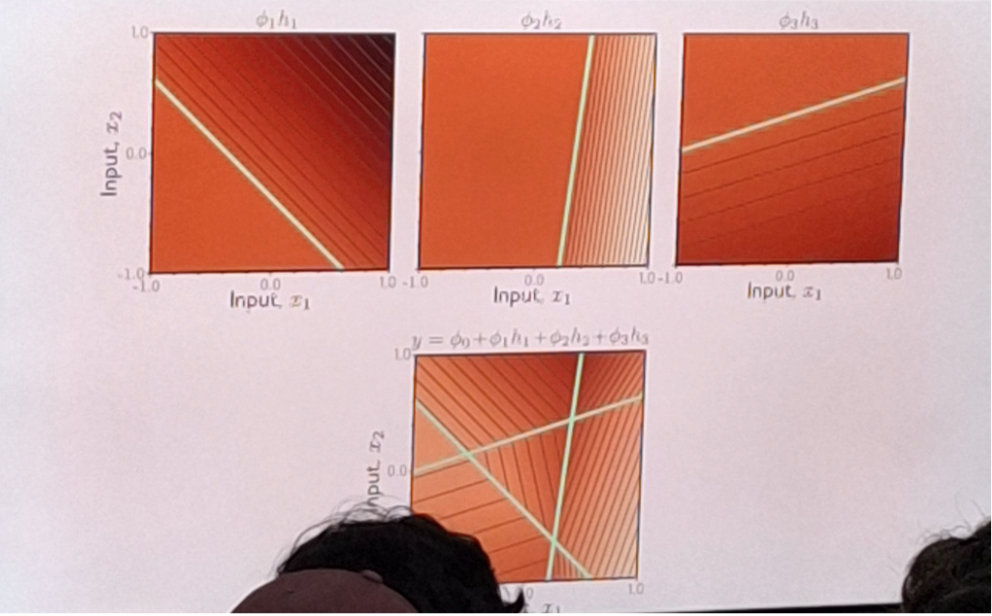
\includegraphics[width=\linewidth]{figures/screenshot.png}
\end{figure} \\
\textbf{Solucion:}
\end{document}
